\documentclass[conference]{IEEEtran}
\IEEEoverridecommandlockouts

\usepackage[british]{babel}
\usepackage[noadjust]{cite}
\usepackage{graphicx}
\usepackage[hyphens]{url}
\usepackage{paralist}
\usepackage{booktabs}
%\usepackage{float}
\usepackage[pdftex,colorlinks=true]{hyperref}

% reduce indent on all paralist environments
%\setdefaultleftmargin{0.5cm}{}{}{}{}{}

\begin{document}

% paper title
\title{Interactions of Language and Multilingual Communities on Twitter}

%Interactions of Language and Multilingual Communities on Twitter during the 2016 Eurovision Song Contest


% author names and affiliations
% use a multiple column layout for up to three different
% affiliations
\author{\IEEEauthorblockN{Nabeel Albishry}
\IEEEauthorblockA{Department of Computer Science\\
University of Bristol\\
Bristol, UK\\
Email: n.albishry@bristol.ac.uk}
\and
\IEEEauthorblockN{Theo Tryfonas}
\IEEEauthorblockA{Department of Civil Engineering\\
University of Bristol\\
Bristol, UK\\
Email: theo.tryfonas@bristol.ac.uk}
\and
\IEEEauthorblockN{Tom Crick}
\IEEEauthorblockA{Department of Computing\\
Cardiff Metropolitan University\\
Cardiff, UK\\
Email: tcrick@cardiffmet.ac.uk}}

% conference papers do not typically use \thanks and this command
% is locked out in conference mode. If really needed, such as for
% the acknowledgment of grants, issue a \IEEEoverridecommandlockouts
% after \documentclass

% use for special paper notices
%\IEEEspecialpapernotice{(Invited Paper)}

% make the title area
\maketitle


\begin{abstract}
Whilst emerging research is providing insight into the factors that
promote the propagation of information in online social networks
following significant events, such as high-profile international
social events. This paper evaluates the extent to which different
language communities engage and interact. We present our analysis of
online interactions in various languages that took place on the social
networking site Twitter during the Eurovision Song Contest in May
2016.

By utilising language information from user profiles
({\emph{N}}=1,226,959) and status updates ({\emph{N}}=7,926,746)
relating to the Contest to identify and categorise communities, we are
able to provide insight into the pattern of their interactions, as
well as constructing their network graphs to shed light on these
multilingual community. The results show that the nature of the event
is reflected on the engagement degree and wider interaction of
communities, as well as showing the participation pattern of
multilingual users. This analysis of language communities may also
help in deciding which group of users to engage with, and hence
increase the chance of influential action when participating on
Twitter conversations.
\end{abstract}

% For peer review papers, you can put extra information on the cover
% page as needed:
% \ifCLASSOPTIONpeerreview
% \begin{center} \bfseries Keywords \end{center}
% \fi
%
% For peerreview papers, this IEEEtran command inserts a page break and
% creates the second title. It will be ignored for other modes.
%\IEEEpeerreviewmaketitle

% tweak these at the end
% \begin{IEEEkeywords}
% Language communities; community structure; information propagation; social networks; Twitter
% \end{IEEEkeywords}


\section{Introduction}\label{intro}

\subsection{Online Social Networks}
 
In recent years, online social networks (OSNs) have been utilised as
means to express ideas and opinions, spread information about events,
or even stimulate and propagate calls for civic engagement and
societal action. Social networking sites such as Twitter, Facebook,
LinkedIn and YouTube have also empowered individuals to promote their
viewpoints and interests -- professional or otherwise -- to a broad
and diverse global audience. The engagement of certain demographics
with social networks offers the opportunity for researchers interested
in observing and interpreting society to apply established theory and
methods to an emerging digital culture.

To satisfy the demand for various types of communities, interactions
and engagement, there are now vast numbers of social media sites and
platforms\footnote{This list is by no means exhaustive:
\url{http://en.wikipedia.org/wiki/List of social networking
websites}}, along with a number of attempted categorisations. By 2018,
there will be an estimated 2.5 billion active social network users (up
from 1.9 billion in 2014); they are producing massive amounts of data
(volume) on a real-time basis (velocity) with implicit sociological
attributes such as beliefs, opinions, sentiments, behaviours,
structures and influences (variety)~\cite{burnap-et-al:2015}. These
data exhibit the key traits of what is now referred to as big data:
volume, velocity and variety~\cite{postsm:2014}. In this age of big
data and an increasingly interconnected digital society, there is a
new challenge -- the application of robust and scalable methods and
tools that can be applied to digitised social behaviour generated via
social networks so as to be able to efficiently analyse big social
data to provide insight into real-world events and
actions~\cite{lazer-et-al:2009,burnap-et-al:2015}.

% Behaviour and interaction have been empirically studied for centuries
% by social scientists, with rigorously applied methods and analyses
% being developed to yield meaningful results.

Recent
work~\cite{blamey-et-al-2012,schwartz-et-al:2013,blamey-et-al-2013,oatley+crick:2014,mostafa-et-al-ai2016}
has analysed what people say on social media to identify distinctive
words, phrases, and topics as functions of known attributes of people
such as gender, age, location, or psychological characteristics. This
can thus be collated and aggregated, inferring gender, age, location
and sentiments, from social media data. Potential negative
implications of these approaches include the fact that they can be
easily applied to large numbers of people or groups in society without
obtaining their explicit consent or even being aware it is being
done. Data-driven commercial companies, governmental entities, or
even one's followers or friends are able to use software to infer
personality and other attributes -- such as sexual orientation or
political affiliations -- that an individual may have decided not to
share~\cite{lambiotte+kosinski:2014,postsm:2014}.

There are various projects that have used Twitter corpora and related
datasets to make predictions about
elections~\cite{tumasjan-et-al:2010}, stock
markets~\cite{zhang-et-al:2011}, and crimes and
policing~\cite{gerber:2014,oatley+crick:2015}. Twitter
played an important role during what was then known as the ``Arab
Spring'', which has been extensively examined in the social network
analysis
domain~\cite{lotan-et-al:2011,howard-et-al:2011,comunello+anzera:2012,wolfsfeld-et-al:2013,bruns-et-al:2013}.
While the use of Twitter data has been demonstrated to provide insight
-- and sociologically relevant demographics~\cite{sloan-et-al:2013} --
into major social and physical events such as
riots~\cite{procter-et-al:2013} and terror
attacks~\cite{burnap-et-al:2014}, often all is not what it may seem;
for instance, many tweets may not a crowd make~\cite{liang-et-al:2013}.

\subsection{Languages and Communities}

Despite the widespread engagement with Twitter globally, little
research has investigated the differences amongst users of various
languages; there is a tendency to assume that the behaviours of
English users generalise to other language
users~\cite{hong-et-al:2011}. Language has featured as a facet of
research on the geographies of Twitter
networks~\cite{takhteyev-et-al:2012}, especially whether offline
geography still matter in online social
networks~\cite{kulshrestha-et-al:2012}. Linguistic-inspired studies
have been done on hashtags~\cite{cunha-et-al:2011}, as well as the
volume and proportional of tweets in English and Arabic, as part of an
analysis of the Arab Spring~\cite{bruns-et-al:2013}. Nevertheless,
language is clearly a vital component of affiliation and discourse on
the web~\cite{zappavigna+martin:2012}, with the creation and curation
of emerging multilingual networks and communities, representing
well-established creative and cultural norms, including for minority
languages such as Welsh~\cite{gj+uj:2013}, as well as investigations
into the economics of linguistic
diversity~\cite{ginsburgh+weber:2011}.


\subsection{Social Network Analysis}

In the social network analysis (SNA) domain, centrality measures
provide the ability to assess network graphs that are constructed from
collected data (for example, tweets). Selection of these centrality
measures is dependent on the goal of the analysis; for example, the
degree of node helps to identify nodes with high number of connections
within the
network~\cite{borgatti+everett:2000,rombach-et-al:2014,liu-et-al:2014}.
In a representation of a real world network, this metric may help to
identify highly connected persons, such as political leaders, sports
stars or celebrities, who are potential ``information
spreaders''~\cite{cha-et-al:2012,borge-holthoefer-et-al:2012,zhang-et-al:2016}.
Centrality measures such as degrees, betweenness, clustering
coefficient, modularity and cliques have been used in many projects to
measure influence or detect the emergence of new
communities~\cite{willis-et-al:2015,oatley+crick:2015}.

Clustering users in communities has been an important analytic factor
in social networking analysis; numerous work has focused on clustering
users based on their locations. However, for the sake of anonymity,
many users tend not to disclose information about their identity, such
as locations~\cite{kang-et-al:2013}. It has also been reported in the
literature that geotagged tweets are generally low in
number~\cite{morstatter-et-al:2013,tan-et-al:2013,kumar-et-al:2014},
the exponential growth in social media over the past decade has been
joined by the rise of location as a central organising
theme~\cite{liang-et-al:2013} of how users engage with online
information services and, more importantly, with each
other~\cite{cheng-et-al:2010,caverlee-et-al:2013}.

\subsection{Users and Location}

It is important to understand how geotagging works in Twitter. The
`place' entity included in a Twitter status does not necessarily
indicate precisely where the actual posting was made, as stated in the
Twitter API
documentation\footnote{\url{https://dev.twitter.com/overview/api/places}}:

\begin{quotation} ``{\emph{Tweets associated with places are not
necessarily issued from that location but could also potentially be
about that location.}}
\end{quotation}

For the sake of anonymity many users tend not to disclose information
about their identity, particularly locations; this has also been
supported by the literature that geotagged tweets are generally low in
number~\cite{kang-et-al:2013}. An alternative location-based option to
consider is based on profile location, but this may not serve the need
for location clustering for a multitude of reasons, especially with a
significant proportion of Twitter users not setting their profile
location~\cite{graham-et-al:2014} (discussed in more detail in
Section~\ref{locations}).

\subsection{Overview of Paper}

The techniques we introduce in this paper are based on language
settings in users' profiles and those for statuses\footnote{The term
`status' is a generic term used to refer to any Twitter post (tweet,
retweet, reply, or quote).}. The remainder of this paper is organised
as follows: Section~\ref{context} introduces the context of the
Eurovision Song Contest case study; in Section~\ref{langcomm} we
present the techniques we have used to identify and analyse language
communities and networks, along with the main results. Finally,
Section~\ref{conclusions} concludes the paper with a wider discussion
and a summary of the potential application of our approach.


\section{Context and Events Timeline}\label{context}

The Eurovision Song Contest ({\emph{Concours Eurovision de la
chanson}}) -- sometimes popularly called Eurovision -- is the
longest-running annual international TV song competition, held,
primarily, among the member countries of the European Broadcasting
Union since 1956. Each participating country submits an original
song to be performed on live television and radio and then casts votes
for the other countries' songs to determine the most popular song in
the competition. The contest has been broadcast every year for sixty
years, and is one of the longest-running television programmes in the
world. It is also one of the most watched non-sporting events in the
world, with audience figures varying in recent years from 100 million
to 600 million globally\footnote{\url{https://www.eurovision.tv}}. The
emergence of social networking in recent years has dramatically
changed the range and scope of audience interaction and engagement,
particularly for different language communities.

The 2016 Eurovision Song
Contest\footnote{\url{https://www.eurovision.tv/page/stockholm-2016/all-participants}}
took place in May in Stockholm, Sweden. There were 32 countries taking
part, with two semi-finals taking place on 12 and 14 May. 26 countries
qualified for the final on 16 May. This year’s contest was perceived
by many commentators to be tense and politically motivated, especially
with Ukraine eventually winning the
final~\cite{telegrapheuroboycott:2016}. Varying analyses see the
contest as being influenced by political conflicts, friendships or
cultural
bias~\cite{ginsburgh+noury:2008,charron:2013,blangiardo+baio:2014,budzinski+pannicke:2016},
with a range of news articles explicitly discussing the possibly
biased results~\cite{telegrapheurobias:2016}.  Twitter activity was
very high throughout the event on the main {\texttt{\#Eurovision}}
hashtag. The participation exceeded 7,900,000 statuses, produced by
1,226,959 users; Figure~\ref{fig:overallactivity} shows the overall
Twitter activity.


\begin{figure}[!htb]
\centering
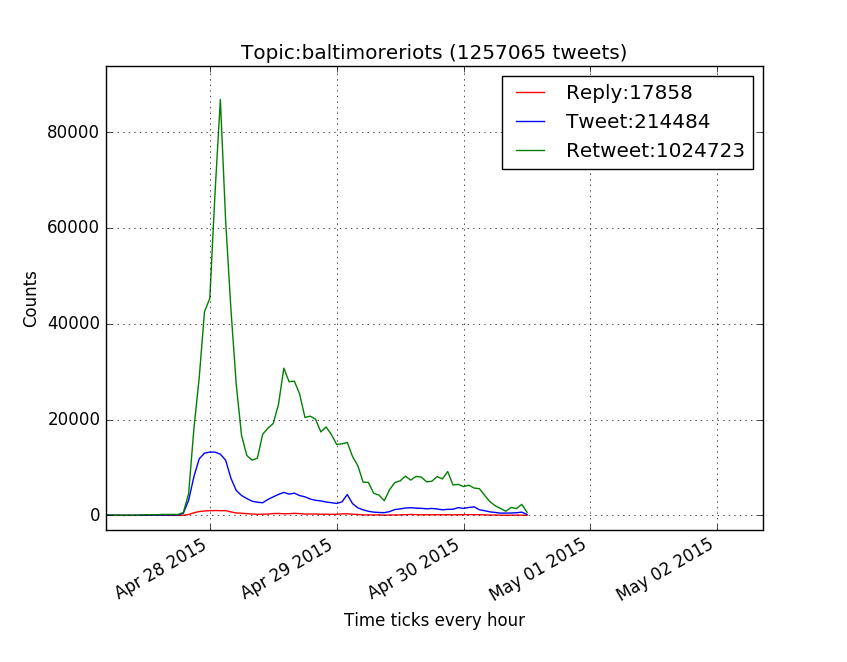
\includegraphics[width=\columnwidth]{images/overallactivity.png}
\caption{Overall activity for {\texttt{\#Eurovision}}.}
\label{fig:overallactivity}
\end{figure}


\section{Language Communities}\label{langcomm}

Preliminary analysis shows that tweets and retweets together account
for c.97\% from the total activity, as shown in
Figure~\ref{fig:overallactivity}. These two subsets can be
representative on their own, without the need to include other
interaction sets, such as replies and quoted tweets. It is important
to note that tweets and retweets are used to measure actions, and
reactions, respectively. However, our analysis will be focusing on
original tweets only and the usage of different languages in this set.

Analysis of language communities begins with two basic techniques. The
first is to classify statuses based on their languages. The status
language is extracted from the `{\emph{lang}}' entity inside status
objects. Language used in posting defines which community the status
was meant for; a tweet written in Turkish, for example, is generally
meant for the Turkish-speaking community. Output from this will be
referred to as `posting communities'. The second approach is to
classify users into different communities based on their profile
languages, regardless of the posting language they used. Output from
this technique will be referred to as `profile communities'. As we
will see in the following sections, a posting community does not
necessarily indicate the profile community for a user.

\subsection{Locations}\label{locations}

As mentioned in Section~\ref{intro}, for the sake of anonymity many
users tend not to disclose information about their identity,
particularly locations; this has also been supported by the literature
that geotagged tweets are generally low in
number~\cite{kang-et-al:2013}. We took the step to verify this claim
in our datasets; in the best cases, the ratio of geotagged tweets did
not exceed 2\%. An alternative location-based option to consider is
based on profile location, but it still does not serve the need for
location clustering for a multitude of reasons. Firstly, we found that
less than 45\% of users have set their profile location, which is in
line with other studies~\cite{graham-et-al:2014}. Secondly, although
Twitter suggests certain presets for setting profile location, users
are given the option to enter any text they wish; this results in a
considerable amount of noise.

\subsection{Profile and Posting Communities}\label{ppcomm}

In the {\texttt{\#Eurovision}} case, there were 49 posting
languages. Table~\ref{tbl:activelangs} shows the top posting languages
accounted for 90\% of original posts (tweets), out of 3,834,937. As
might be expected, the English was the most used posting
language. Interestingly, the results show that the language of 142,721
(3.72\%) statuses could not be identified. When investigated further,
c.40\% of these statuses did not contain much text other than
hashtags, user mentions or URLs. Although this category shows an
interesting case in which qualitative content analysis could be
involved, it is beyond the scope of this study and will not be
addressed here.


\begin{table}[!htb]
\centering
\begin{tabular}{@{}lc}
\toprule
\textbf{Language} & \textbf{\%} \\ 
\midrule
{\emph{en}} & 45.90 \\
{\emph{es}} & 17.24 \\
{\emph{ru}} & 8.99 \\
{\emph{fr}} & 6.20 \\
{\emph{und}} & 3.72 \\
{\emph{nl}} & 3.71 \\
{\emph{de}} & 3.19 \\
{\emph{it}} & 2.85 \\ 
\bottomrule
\end{tabular}
\caption{Most active profile language
  communities, accounting for 90\% of original tweets}
\label{tbl:activelangs}
\end{table}


In total, 1,226,959 users interacted with the {\texttt{\#Eurovision}}
hashtag. In terms of their profile languages, they formed 50
communities. Table~\ref{tbl:profcomms} shows the profile communities
from the top 90\% of all users. Unlike status language, profile
language relies on the user to pick a language for their Twitter
profile settings. In general, the default value of this option is the
initial placeholder text ``{\emph{Select Language...}}'' or a
translated version that might provide hints regarding the user
language community. In our dataset, we found that all users had
selected a language and no users with the default value.


\begin{table}[!htb]
\centering
\begin{tabular}{@{}lc}
\toprule
\textbf{Community} & \textbf{\%} \\ 
\midrule
{\emph{en}} & 47.06 \\
{\emph{es}} & 20.37 \\
{\emph{fr}} & 8.00 \\
{\emph{ru}} & 7.07 \\
{\emph{de}} & 3.539 \\
{\emph{nl}} & 3.31 \\
{\emph{it}} & 2.25 \\ 
\bottomrule
\end{tabular}
\caption{Profile communities, for top 90\% of users}
\label{tbl:profcomms}
\end{table}


\subsection{Profile-Posting Analysis}

From the previous two tables, we can see some similarities between the
posting and profile communities. Taking an exceptional case as an
example, we can see that although the French profile community had
more presence, the Russian posting community is larger by 2.79\%. A
simple explanation would be that the Russian profile community was
relatively more active than French due to the focus on related
countries; another reason could be the participation of non-Russian
profiles using the Russian language for posting. To investigate this,
we investigated the contribution of profile communities to the Russian
posting community. The result in Table~\ref{tbl:russian} shows profile
communities that resulted in more than 95\% of activity in this
posting community.


\begin{table}[!htb]
\centering
\begin{tabular}{@{}lc}
\toprule
\textbf{Community} & \textbf{\%} \\ 
\midrule
{\emph{ru}} & 91.25 \\
{\emph{en}} & 7.26 \\
\bottomrule
\end{tabular}
\caption{Active profile communities within the Russian posting community}
\label{tbl:russian}
\end{table}


As we can see in this example, posts in Russian were not merely
appearing from the Russian profile community. This show one way of
exploring relationships between profile and posting communities,
especially if we are interested in particular communities.

Another approach is to explore the posting behaviour of one particular
community. When considering certain profile communities, there is a
tendency to assume that communities only post in languages that are
the same as their profile language. To examine this assumption, we
investigated participation of `{\emph{en}}' profiles, as they form
nearly 50\% of users. In total, there were 1,841,205 posts from this
community, 81\% of which were posted in `{\emph{en}}', 15.4\% in other
languages, and 3.62\% were not identified. Table~\ref{tbl:enpartlangs}
lists the top 95\% posting languages used by this profile community.


\begin{table}[!htb]
\centering
\begin{tabular}{@{}lc}
\toprule
\textbf{Language} & \textbf{\%} \\ 
\midrule
{\emph{en}} & 80.99 \\
{\emph{und}} & 3.62 \\
{\emph{es}} & 2.69 \\
{\emph{nl}} & 2.39 \\
{\emph{fr}} & 1.39 \\
{\emph{ru}} & 1.36 \\
{\emph{de}} & 0.97 \\
{\emph{it}} & 0.87 \\ 
{\emph{el}} & 0.86 \\ 
\bottomrule
\end{tabular}
\caption{Top 95\% of participation languages from `{\emph{en}}' profiles}
\label{tbl:enpartlangs}
\end{table}


\subsection{Language Diversity}

By observing the language diversity of profile communities, we aim to
measure language diversity of the topic in general, as well as
investigating which community plays a key role in bridging different
profile communities. Diversity in this context means how many posting
languages were used from each profile community, and to what extent
they used their own language, as well as other languages.  The general
language diversity of the topic is c.17\%, while 3.72\% were not
identified. All of the 50 profile communities used different languages
in posting. Interestingly, 16 out of those communities did not use
their own language, they were low in participation though. Moreover,
in terms of using different languages, we found that 32 communities
scored at least 50\% out of their tweets. We noticed that posting from
small profile communities may affect the overall language diversity of
the topic. Referring to the top profile communities discussed in
Section~\ref{ppcomm}, Table~\ref{tbl:diversity} shows their
diversity by percentage. The Russian profile community is again an
interesting case, as it scored the least diverse profile amongst all
the 50 communities although it comes fourth in number of users.


\begin{table}[!htb]
\centering
\begin{tabular}{@{}lc}
\toprule
\textbf{Language} & \textbf{\%} \\ 
\midrule
{\emph{de}} & 34.27 \\
{\emph{nl}} & 32.78 \\
{\emph{it}} & 18.49 \\ 
{\emph{fr}} & 16.65 \\
{\emph{en}} & 15.39 \\
{\emph{es}} & 10.13 \\
{\emph{ru}} & 7.93 \\
\bottomrule
\end{tabular}
\caption{Diversity of the top profile communities}
\label{tbl:diversity}
\end{table}


\subsection{Multilingual Communities}

In this section, we group users based on their relationship with
posting communities, regardless of their profile language. For
example, a user posting in both `{\emph{en}}' and `{\emph{fr}}' will
be classified as bilingual, and so on. Based on this grouping
technique, with the `{\emph{und}}' lang category eliminated, we
identified 20 sets. The smallest two groups consist of one user each,
who posted in 22 and 25 different languages.  As we can see in
Figure~\ref{fig:multilingual}, monolingual users scored about 85\% of
all users, creating 47\% of the total original posts. The also shows
that users and their activity decrease as number of languages used
increase.


\begin{figure}[!htb]
\centering
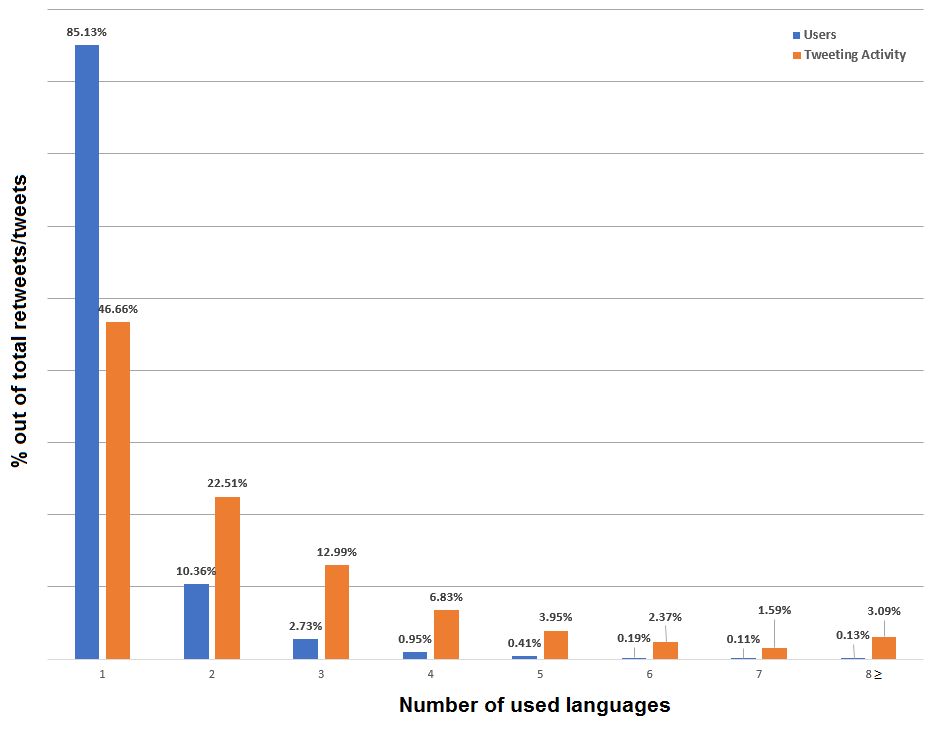
\includegraphics[width=\columnwidth]{images/multilingualcommunities.png}
\caption{Multilingual communities and their associated activities.}
\label{fig:multilingual}
\end{figure}


A closer look at the behavior of these communities shows that, in
general, activity per user increases as number of used languages
increase, as shown in
Figure~\ref{fig:multilingualpostsperuser}. Although we cannot conclude
that there is a correlation between high multilingualism and
illegitimacy of accounts, this would be an interesting further topic
to investigate.


\begin{figure}[!htb]
\centering
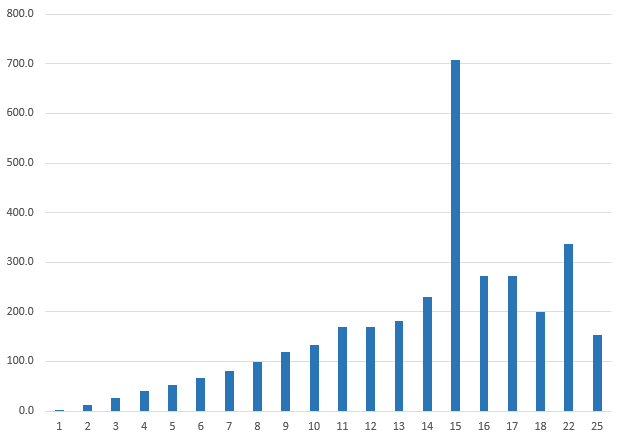
\includegraphics[width=\columnwidth]{images/multilingualpostsperuser.png}
\caption{Average number of posts per user for multilingual communities.}
\label{fig:multilingualpostsperuser}
\end{figure}


\section{Conclusions}\label{conclusions}

This paper presented a study in identifying languages used, language
and multilingual communities, and their engagement and interactions on
the Twitter platform with respect to real world events, in this
instance using the Eurovision Song Contest in May 2016.  As we
discussed in Section~\ref{langcomm}, there is a positive relationship
between size of profile and posting communities. We have also showed
that a large number in participating profile community does not
necessarily imply high language diversity, and that diversity may
results from small profile community.

We also presented the structure of multilingual communities and their
activity. Although most users may use their own profile language in
posting, most of the activity came from multilingual users. In a few
cases, users may use a significant number of languages, up to 25
different languages. These extreme cases may be interesting to
investigate for possible spammer/false account detection or for
sociolinguistics in more moderate cases.

The method we presented here can be used in identifying how
communities interact with one another, which ones are most active,
which languages are mostly used, and at what time. Moreover, within
certain contexts, the order of applying these two classifications
(posting and profile) will generate results in different
perspectives. For example, taking one profile community and dividing
it into different posting communities shows the number of languages
this community may use, and hence degree of openness and
reachability. A possible scenario for governments, politicians or
campaigners would be to use this method to measure to what extent
other languages are used within a profile community. It may also show
how users associate themselves with one community in their profile
while using other languages. Monitoring unusual activity for secondary
languages, in multilingual communities, may help to uncover important
messages or opinions that could not be openly expressed, for a variety
of reasons, to the rest of the profile community. Applying these
techniques on data pouring from the Twitter Stream
API\footnote{\url{https://dev.twitter.com/streaming/overview}} would
be applicable to a wide number of domains. For example, these methods
can be used in social network marketing and publicity to increase the
probability of influential posts. In practice, for a given
{\texttt{\#<Brand>}}, by monitoring the activity of different language
community, one can decide the time to post well-tailored tweets
targeting certain communities.

For future work, we plan to have a deeper look at how multilingual
communities participate and their reaction networks. We believe that
differentiation between endorsements (e.g. retweets) and other
reactions may provide further insight into the networks and
communities. Furthermore, we will apply the methods presented in this
paper on other high-profile event/discussion datasets in different
domains or contexts, such as for sports and humanitarian/civil rights
actions.


\section*{Acknowledgment}
\addcontentsline{toc}{section}{Acknowledgment}

This work has been supported by a doctoral research scholarship for
Nabeel Albishry from King Abdulaziz University, Kingdom of Saudi
Arabia.


%\newpage

% trigger a \newpage just before the given reference
% number - used to balance the columns on the last page
% adjust value as needed - may need to be readjusted if
% the document is modified later
\IEEEtriggeratref{33}
% The "triggered" command can be changed if desired:
%\IEEEtriggercmd{\enlargethispage{-5in}}

% references section
\bibliographystyle{IEEEtran}
\bibliography{icc2017}

% that's all folks
\end{document}


